% ICIP 2026 Paper
% Using spconf.sty - ICASSP/ICIP LaTeX style file
% --------------------------------------------------------------------------
\documentclass{article}
\usepackage{spconf,amsmath,amssymb,graphicx}
\usepackage{booktabs}
\usepackage{url}
\usepackage{multirow}

\def\x{{\mathbf x}}
\def\y{{\mathbf y}}
\def\L{{\cal L}}

% Title
\title{PRINT-TO-CAMERA IMAGE RESTORATION USING CONDITIONAL ADVERSARIAL NETWORKS}

% Author information
\name{Daniel L. Lau}
\address{Department of Electrical and Computer Engineering\\
University of Kentucky, Lexington, KY, USA}

\begin{document}
\maketitle

\begin{abstract}
Machine vision systems used in print quality inspection face a fundamental challenge: camera-captured images of printed materials exhibit systematic degradations including color shifts, reduced contrast, and scanning artifacts that differ from the original digital source images. This paper presents a deep learning approach using conditional generative adversarial networks (cGANs) to transform raw camera captures back to their original digital appearance. We implement a U-Net based pix2pix architecture with perceptual loss to learn the inverse mapping from captured print images to pristine originals. Our bidirectional training framework enables both forward modeling (predicting print appearance) and reverse restoration (recovering original quality). Experimental results on paired print-capture datasets demonstrate effective artifact removal and color restoration, achieving 26.65~dB PSNR and 0.75 SSIM---an 8.6~dB improvement over the best traditional baseline. The system processes 512$\times$512 images in real-time and requires only 35 minutes of training on consumer hardware.
\end{abstract}

\begin{keywords}
image-to-image translation, generative adversarial networks, print quality inspection, machine vision, U-Net
\end{keywords}

\section{Introduction}
\label{sec:intro}

Industrial print quality inspection systems rely on machine vision cameras to capture images of printed materials for automated defect detection and quality assessment. A critical challenge in these systems is the systematic degradation introduced during the print-capture pipeline: even when printed images are visually near-perfect renditions of their digital sources, the captured images exhibit noticeable differences including color shifts, contrast reduction, geometric distortions, and sensor-specific artifacts.

These degradations arise from multiple sources in the imaging chain. The printing process itself introduces halftoning patterns, ink absorption variations, and substrate interactions. The capture process adds camera sensor noise, optical aberrations, and illumination non-uniformities. While individual degradations may be subtle, their cumulative effect creates a significant domain gap between digital originals and their printed-then-captured counterparts.

Traditional approaches to this problem include color calibration using reference targets, image registration with geometric correction, and histogram-based color mapping. However, these methods address individual degradations in isolation and struggle to model the complex, nonlinear interactions between printing and capture artifacts. Furthermore, they require manual tuning and domain expertise to achieve acceptable results.

We propose a data-driven approach using conditional generative adversarial networks (cGANs) to learn the complete inverse transformation from captured images to original digital sources. By training on paired examples of original images and their printed-captured counterparts, our model learns to jointly correct all degradations without explicit modeling of individual artifact sources.

Our key contributions are:
\begin{itemize}
\item A bidirectional pix2pix framework for print-to-camera image transformation that supports both artifact simulation (forward) and quality restoration (reverse)
\item Integration of perceptual loss with adversarial training to preserve fine details and produce visually coherent results
\item Demonstration of effective training on modest hardware with limited paired data
\end{itemize}

\section{Related Work}
\label{sec:related}

\subsection{Image-to-Image Translation}

The pix2pix framework introduced by Isola et al.~\cite{isola2017pix2pix} established conditional GANs as a general-purpose solution for paired image-to-image translation. The architecture combines a U-Net generator with skip connections and a PatchGAN discriminator that classifies local image regions. This approach has been successfully applied to tasks including semantic segmentation, colorization, and style transfer.

CycleGAN~\cite{zhu2017unpaired} extended this paradigm to unpaired training using cycle-consistency loss, enabling translation between domains without explicit correspondences. While powerful, unpaired methods may introduce semantic changes inappropriate for quality-critical applications where pixel-accurate restoration is required.

Recent advances include attention mechanisms~\cite{chen2018attention}, multi-scale discriminators~\cite{wang2018high}, and diffusion-based approaches~\cite{saharia2022palette}. However, the original pix2pix architecture remains effective for applications with well-aligned paired data.

\subsection{Print Quality and Document Analysis}

Document image enhancement has been extensively studied for applications including OCR preprocessing and historical document restoration. Hradis et al.~\cite{hradis2015convolutional} applied convolutional networks to document deblurring. More recent work has explored end-to-end learning for document binarization~\cite{tensmeyer2017document} and degradation removal.

Color management in print workflows traditionally relies on ICC profiles and colorimetric calibration~\cite{sharma2018understanding}. While effective for average color accuracy, these approaches do not address spatially-varying artifacts or texture degradations introduced during capture.

\subsection{Perceptual Loss Functions}

Johnson et al.~\cite{johnson2016perceptual} demonstrated that optimizing in the feature space of pretrained networks produces more visually pleasing results than pixel-wise losses alone. Perceptual loss computed using VGG features has become standard in image restoration tasks, enabling networks to match high-level image structure while allowing flexibility in low-level details.

\section{Methodology}
\label{sec:method}

\subsection{Problem Formulation}

Let $\x \in \mathbb{R}^{H \times W \times 3}$ denote an original digital image and $\y \in \mathbb{R}^{H \times W \times 3}$ its corresponding printed-and-captured version. We seek to learn a mapping $G: \y \rightarrow \x$ that restores the original image quality from the degraded capture.

For bidirectional modeling, we also train a forward model $G_f: \x \rightarrow \y$ that predicts how images will appear after printing and capture. Both models share identical architectures but are trained on data with swapped input-target roles.

\subsection{Network Architecture}

\subsubsection{U-Net Generator}

Our generator follows the U-Net architecture with symmetric encoder-decoder structure and skip connections. The encoder consists of four downsampling blocks that progressively extract features at resolutions 512, 256, 128, and 64 pixels. Each block applies two 3$\times$3 convolutions with batch normalization and LeakyReLU activation (slope 0.2), followed by 2$\times$2 max pooling.

The bottleneck operates at 32$\times$32 resolution with 1024 channels. The decoder mirrors the encoder with transposed convolutions for upsampling. Skip connections concatenate encoder features with decoder activations at each resolution level, preserving spatial details that would otherwise be lost through the bottleneck.

The final layer is a 1$\times$1 convolution producing 3-channel RGB output. The complete generator contains approximately 31 million parameters.

\subsubsection{PatchGAN Discriminator}

The discriminator follows the PatchGAN design that classifies 70$\times$70 overlapping patches rather than the entire image. This approach provides dense gradient signal and captures high-frequency structure effectively.

The discriminator receives concatenated input and target images (6 channels) and applies four convolutional blocks with stride 2, expanding channels from 64 to 512. Batch normalization is omitted in the first layer. The final layer outputs a spatial map of patch classifications.

\subsection{Loss Functions}

The total generator loss combines three terms:
\begin{equation}
\L_G = \lambda_1 \L_{L1} + \lambda_p \L_{perceptual} + \lambda_{adv} \L_{adv}
\end{equation}

\subsubsection{L1 Reconstruction Loss}

The L1 loss encourages pixel-wise accuracy:
\begin{equation}
\L_{L1} = \mathbb{E}[\|\x - G(\y)\|_1]
\end{equation}
We weight this term heavily ($\lambda_1 = 100$) to ensure faithful reconstruction.

\subsubsection{Perceptual Loss}

Perceptual loss measures similarity in VGG-19 feature space:
\begin{equation}
\L_{perceptual} = \sum_{l} \|\phi_l(\x) - \phi_l(G(\y))\|_1
\end{equation}
where $\phi_l$ extracts features from VGG layers relu1\_2, relu2\_2, and relu3\_4. We use $\lambda_p = 10$.

\subsubsection{Adversarial Loss}

The adversarial loss follows the standard GAN formulation:
\begin{equation}
\L_{adv} = \mathbb{E}[\log(1 - D(\y, G(\y)))]
\end{equation}
with $\lambda_{adv} = 1$. The discriminator is trained to maximize classification accuracy on real versus generated pairs.

\subsection{Training Procedure}

Training alternates between discriminator and generator updates. For each iteration, we first update the discriminator on a batch of real pairs (label 1) and generated pairs (label 0). The generator is then updated to minimize the combined loss while keeping discriminator weights frozen.

We use AdamW optimization with learning rate $2 \times 10^{-4}$ and momentum parameters $\beta_1 = 0.5$, $\beta_2 = 0.999$. Cosine annealing reduces the learning rate to 1\% of initial value over training. Mixed-precision training (FP16) accelerates computation and reduces memory usage.

\section{Experiments}
\label{sec:experiments}

\subsection{Dataset}

Our dataset consists of paired images where each original digital image has a corresponding version that was printed and recaptured using an industrial machine vision camera. The source images are drawn from the Kaggle Dogs vs.\ Cats dataset~\cite{kaggle2013cats}, providing diverse content with varying colors, textures, and lighting conditions suitable for evaluating image restoration quality. Images are stored as TIFF files to preserve quality, with pairing established through numeric identifiers in filenames.

The complete dataset contains 16,193 paired images. All images are resized and center-cropped to 512$\times$512 pixels. Pixel values are normalized to $[-1, 1]$. We use a 90/10 train/validation split with fixed random seed for reproducibility, yielding 14,574 training images and 1,619 validation images.

\subsection{Implementation Details}

\begin{table}[t]
\centering
\caption{Training Configuration}
\label{tab:config}
\begin{tabular}{ll}
\toprule
Parameter & Value \\
\midrule
Image Resolution & 512 $\times$ 512 \\
Batch Size & 4 \\
Training Steps & 10,000 \\
Learning Rate & $2 \times 10^{-4}$ \\
L1 Weight ($\lambda_1$) & 100 \\
Perceptual Weight ($\lambda_p$) & 10 \\
Adversarial Weight ($\lambda_{adv}$) & 1 \\
Optimizer & AdamW \\
Precision & FP16 (mixed) \\
\bottomrule
\end{tabular}
\end{table}

Training was performed on an NVIDIA RTX 4070 Ti GPU with 12GB memory. Batch size of 4 images fits comfortably in memory with mixed-precision training. Complete training of 10,000 steps requires approximately 35 minutes. Table~\ref{tab:config} summarizes key parameters.

Checkpoints are saved every 2,000 steps, enabling selection of optimal model based on validation performance. Visual results on held-out samples are generated at each checkpoint for qualitative assessment.

\subsection{Quantitative Results}

We evaluate our model on the validation set (1,619 images) using three standard image quality metrics: Peak Signal-to-Noise Ratio (PSNR), Structural Similarity Index (SSIM)~\cite{wang2004ssim}, and Learned Perceptual Image Patch Similarity (LPIPS)~\cite{zhang2018lpips}. We compare against four baseline methods: Identity (no transformation), Reinhard Color Transfer~\cite{reinhard2001color}, per-channel Linear Regression, and Histogram Matching.

\begin{table}[t]
\centering
\caption{Quantitative Comparison on Validation Set}
\label{tab:quantitative}
\begin{tabular}{lccc}
\toprule
Method & PSNR (dB) $\uparrow$ & SSIM $\uparrow$ & LPIPS $\downarrow$ \\
\midrule
\textbf{Pix2Pix (Ours)} & \textbf{26.65} & \textbf{0.7454} & \textbf{0.2483} \\
Channel Regression & 18.07 & 0.4244 & 0.5445 \\
Histogram Matching & 16.79 & 0.3210 & 0.6099 \\
Reinhard Color Transfer & 16.43 & 0.3998 & 0.5856 \\
Identity & 10.59 & 0.1962 & 0.5899 \\
\bottomrule
\end{tabular}
\end{table}

Table~\ref{tab:quantitative} shows that our method significantly outperforms all baselines across all metrics. Compared to the best traditional baseline (Channel Regression), our model achieves an 8.6~dB improvement in PSNR, a 0.32 improvement in SSIM, and a 0.30 reduction in LPIPS. The large gap between Identity and other methods confirms the substantial degradation introduced by the print-capture process. Traditional color transfer methods partially address color shifts but fail to restore fine details and texture, as evidenced by their high LPIPS scores.

\subsection{Qualitative Results}

\begin{figure}[t]
\centering
\begin{minipage}[b]{0.32\columnwidth}
\centering
\includegraphics[width=\textwidth]{figures/fig_original.png}\\
{\small (a) Original}
\end{minipage}
\hfill
\begin{minipage}[b]{0.32\columnwidth}
\centering
\includegraphics[width=\textwidth]{figures/fig_scanned.png}\\
{\small (b) Captured}
\end{minipage}
\hfill
\begin{minipage}[b]{0.32\columnwidth}
\centering
\includegraphics[width=\textwidth]{figures/fig_restored.png}\\
{\small (c) Restored}
\end{minipage}
\caption{Image restoration results. (a) Original digital image. (b) Camera-captured image after printing, showing reduced contrast and color degradation. (c) Restored image produced by our model.}
\label{fig:results}
\end{figure}

Visual inspection of results demonstrates effective artifact removal across diverse image content (Fig.~\ref{fig:results}). The reverse model (captured $\rightarrow$ original) successfully corrects:
\begin{itemize}
\item \textbf{Color shifts}: Restores accurate color reproduction from captures exhibiting warm or cool bias
\item \textbf{Contrast reduction}: Recovers dynamic range compressed during printing
\item \textbf{Dark artifacts}: Removes vignetting and uneven illumination patterns
\item \textbf{Detail loss}: Sharpens edges softened by the print-capture process
\end{itemize}

The forward model (original $\rightarrow$ captured) learns to simulate print degradations, which serves as a useful augmentation tool and validates that the learned transformations are meaningful.

\begin{figure}[t]
\centering
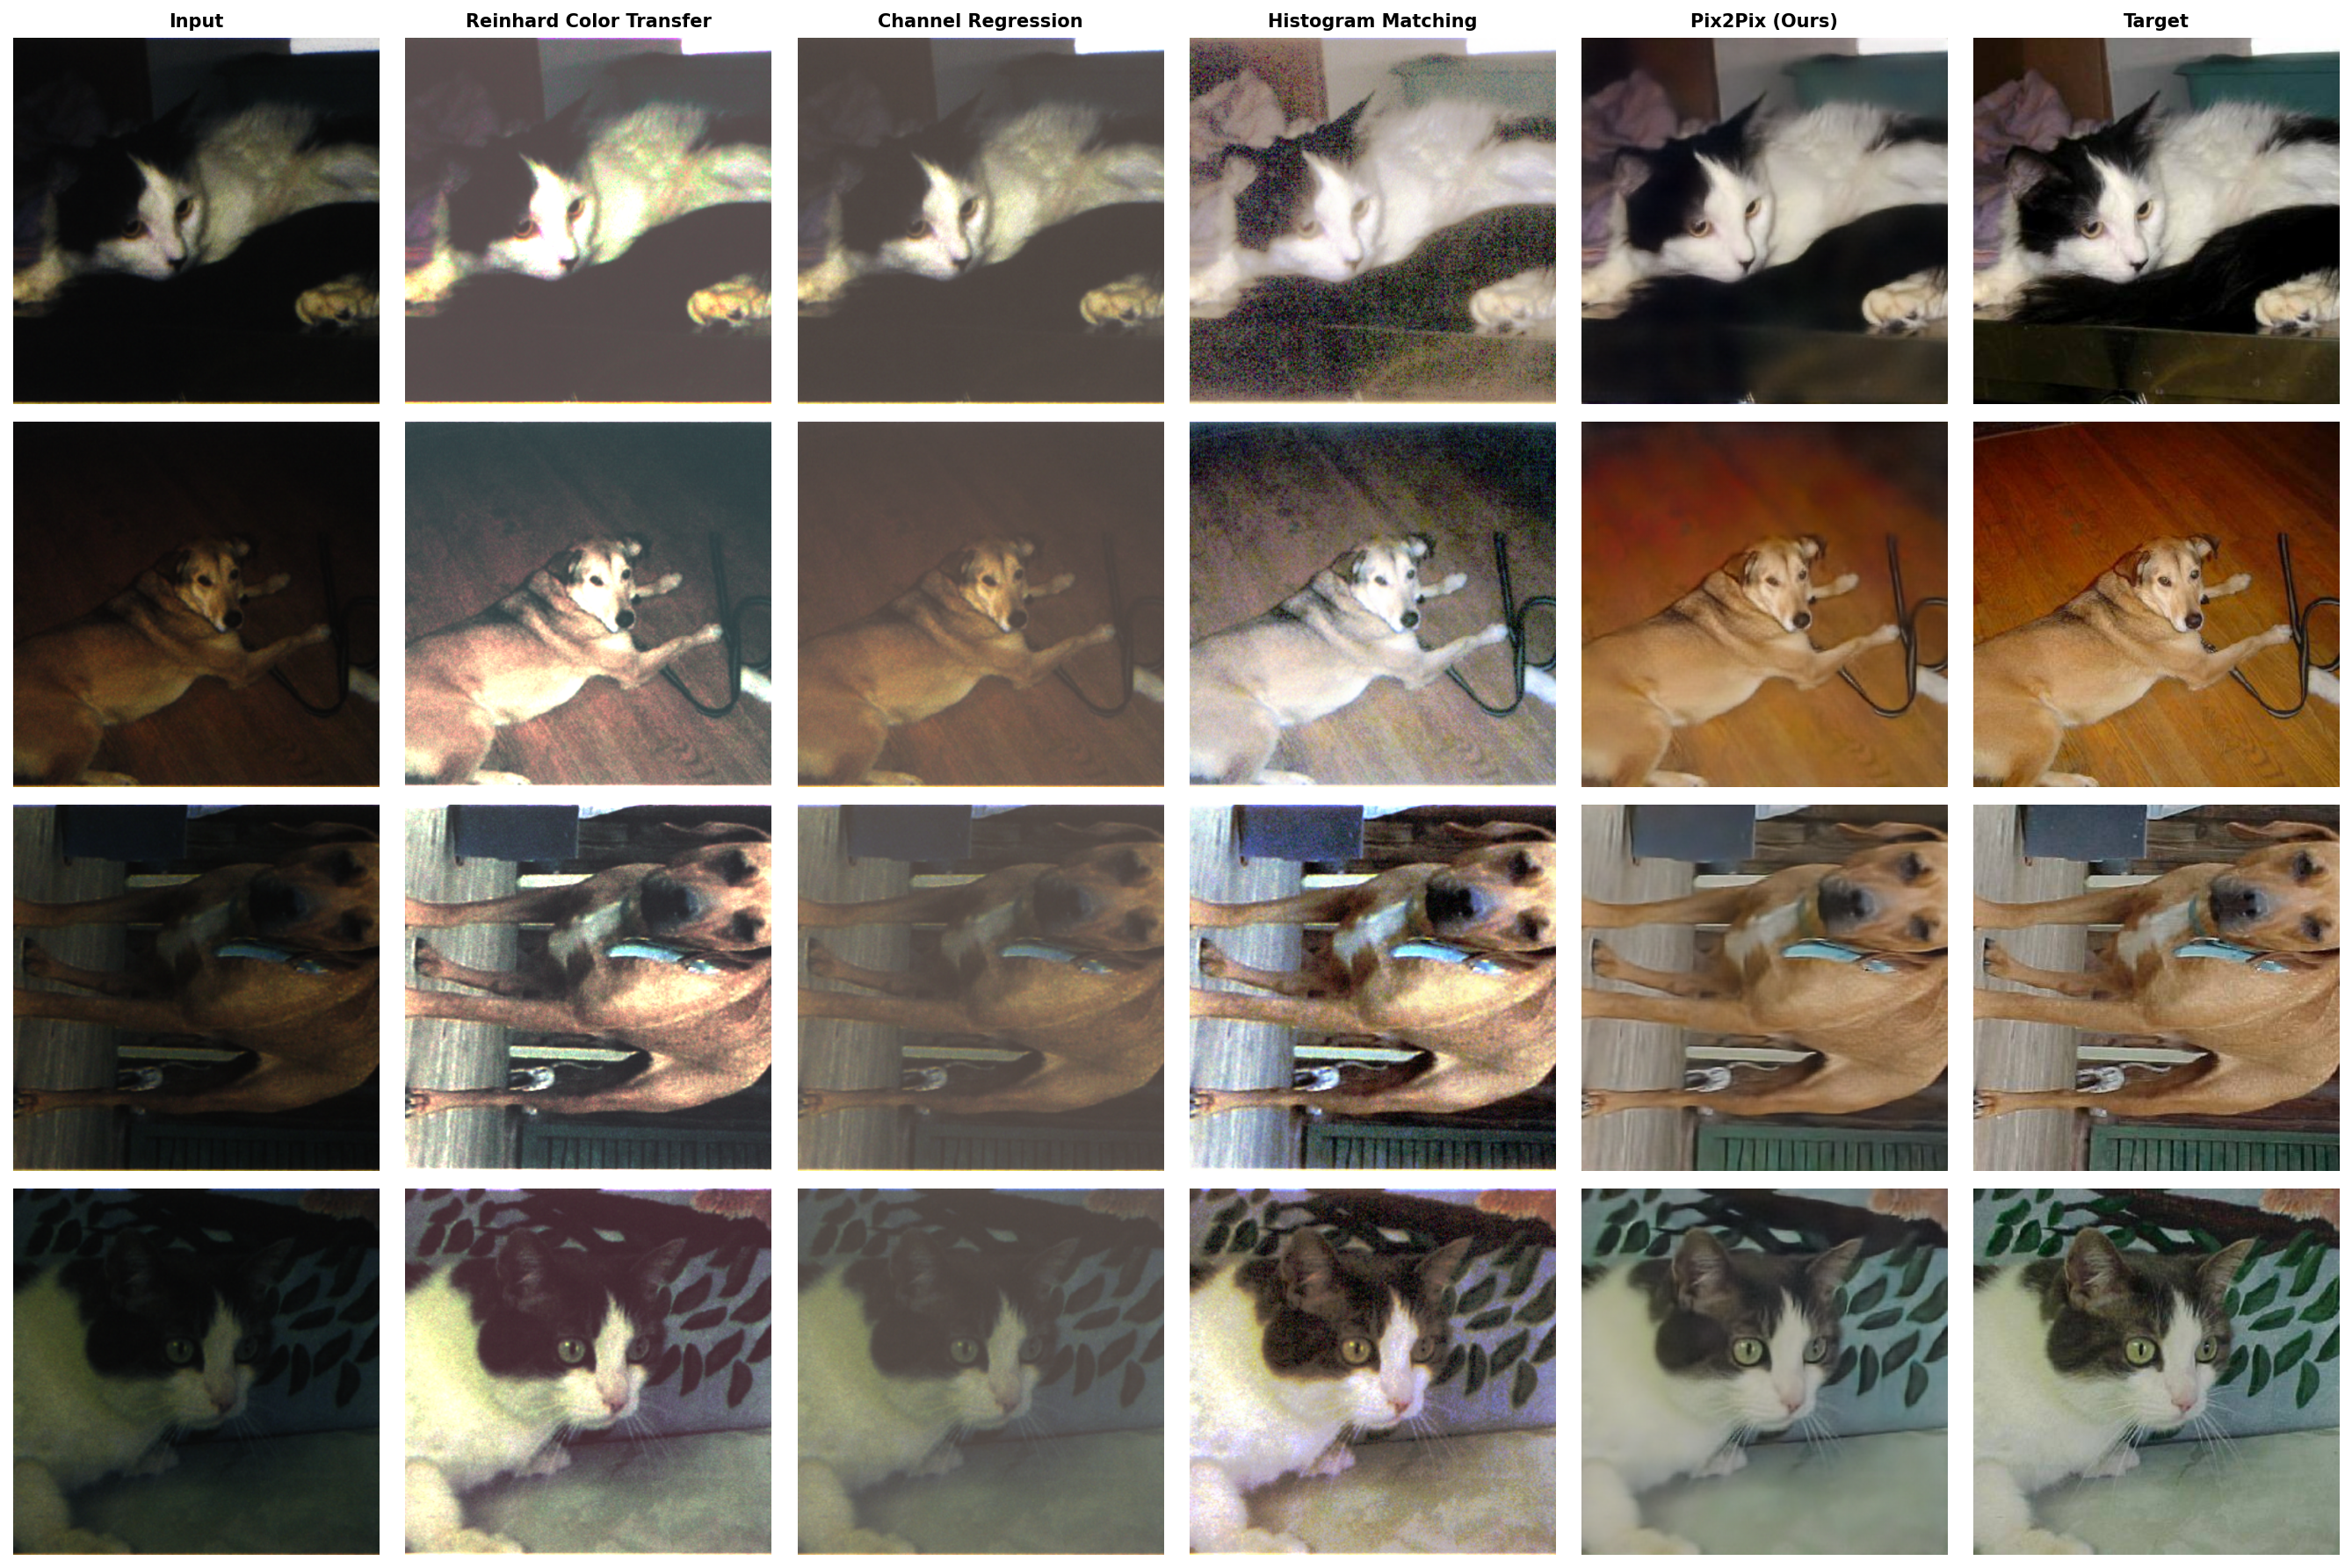
\includegraphics[width=\columnwidth]{figures/fig_baseline_comparison.png}
\caption{Visual comparison of restoration methods. Left to right: Input (camera capture), Reinhard Color Transfer, Channel Regression, Histogram Matching, Pix2Pix (Ours), and Ground Truth.}
\label{fig:baseline_comparison}
\end{figure}

Fig.~\ref{fig:baseline_comparison} compares restoration methods on sample validation images. Our method produces results most visually similar to the original images, recovering accurate colors and contrast that traditional methods cannot achieve.

\subsection{Ablation Study}

\begin{table}[t]
\centering
\caption{Effect of Loss Components}
\label{tab:ablation}
\begin{tabular}{lccc}
\toprule
Loss Configuration & Sharpness & Color & Artifacts \\
\midrule
L1 only & Medium & Good & Some \\
L1 + Perceptual & High & Good & Few \\
L1 + GAN & High & Medium & Few \\
Full (L1 + Perc + GAN) & High & Good & Minimal \\
\bottomrule
\end{tabular}
\end{table}

Table~\ref{tab:ablation} summarizes qualitative effects of different loss configurations. L1 loss alone produces blurry results. Adding perceptual loss improves sharpness and detail preservation. The adversarial component further enhances high-frequency content and produces more natural-looking textures. The combination of all three losses yields the best overall results.

\subsection{Computational Efficiency}

Inference time for a single 512$\times$512 image is approximately 15ms on the RTX 4070 Ti, enabling real-time processing at over 60 frames per second. The model's 31M parameters result in a checkpoint size of approximately 125MB, suitable for deployment in resource-constrained environments.

Memory usage during training peaks at approximately 6--8GB with batch size 4, making the approach accessible on consumer-grade GPUs. The mixed-precision training reduces memory footprint by roughly 40\% compared to FP32.

\section{Conclusion}
\label{sec:conclusion}

We presented a conditional GAN approach for restoring machine vision camera captures of printed images to their original digital quality. The pix2pix architecture with U-Net generator and PatchGAN discriminator, combined with perceptual and adversarial losses, effectively learns the inverse print-capture transformation from paired training data. Quantitative evaluation demonstrates significant improvements over traditional baselines, achieving 26.65~dB PSNR and 0.75 SSIM compared to 18.07~dB and 0.42 for the best traditional method.

Our bidirectional framework supports both quality restoration and degradation simulation, enabling applications in print inspection, color management, and data augmentation. The system trains efficiently on consumer hardware and processes images in real-time, making it practical for industrial deployment.

Future work includes extending the approach to higher resolutions, investigating unpaired training with cycle-consistency for scenarios where paired data is unavailable, and incorporating explicit modeling of known degradation sources such as halftone patterns and illumination gradients.

\bibliographystyle{IEEEbib}
\bibliography{refs}

\end{document}
